% !TeX program = xelatex
% !TeX encoding = UTF-8
% !TeX TXS-program:compile = txs:///xelatex | txs:///xelatex
\documentclass[aspectratio=169, table, 12pt]{beamer}

% Preamble bersama seluruh slide mata kuliah ini.
% Dipanggil dari slides/sessionXX/sessionXX.tex tepat sesudah baris
% \documentclass[aspectratio=169, table, 12pt]{beamer}
% Paket tambahan yang hanya dibutuhkan satu sesi ditulis di berkas sesi itu.

\usepackage{colortbl}
\usepackage{xcolor}
\usepackage{listings}
\usepackage{tabularx}
\usepackage{booktabs}
\usepackage{tikz}
\usepackage{pgfplots}
\usepackage{fontspec}
\usepackage[english,bahasai]{babel}
\pgfplotsset{compat=1.18}
\usetikzlibrary{arrows.meta, positioning, calc, fit, shapes.geometric,
  shapes.multipart, backgrounds, matrix, chains, trees}

\makeatletter
\def\input@path{{../theme/}}
\makeatother
\graphicspath{{../theme/}{../../figures/}}
% Stub symlink Windows memakai tema cadangan sampai aset institusi tersedia.
\IfFileExists{../theme/beamerthemePradita.sty}{%
  \usetheme{Pradita}
}{%
  \usetheme{Madrid}
  \setmainfont{TeX Gyre Heros}
  \setsansfont{TeX Gyre Heros}
  \setbeamertemplate{navigation symbols}{}
}

\definecolor{praditagreen}{RGB}{37, 113, 71}
\setbeamercolor{structure}{fg=praditagreen}
\setbeamercolor{palette primary}{bg=praditagreen,fg=white}
\setbeamercolor{palette secondary}{bg=praditagreen!80!black,fg=white}
\setbeamercolor{palette tertiary}{bg=praditagreen!60!black,fg=white}
\setbeamerfont{frametitle}{size=\large}
\setbeamertemplate{caption}[numbered]

% Ukuran header mengikuti teks agar judul panjang tidak menabrak logo.
\setbeamercolor{frametitle}{bg=white,fg=black}
\setbeamertemplate{frametitle}{%
  \begin{beamercolorbox}[wd=\paperwidth,sep=0.2cm]{frametitle}
    \begin{minipage}[c]{0.77\paperwidth}
      \raggedright\fontsize{16}{18}\selectfont\bfseries\insertframetitle
      \ifx\insertframesubtitle\empty\else
        \par\small\mdseries\insertframesubtitle
      \fi
    \end{minipage}\hfill
    \begin{minipage}[c]{0.15\paperwidth}
      \IfFileExists{../theme/classFiles/logo_universitas.png}{%
        
\includegraphics[width=\linewidth]{../theme/classFiles/logo_universitas.png}%
      }{}
    \end{minipage}
  \end{beamercolorbox}
}
\setbeamertemplate{footline}{%
  \ifnum\value{framenumber}>1
    \begin{beamercolorbox}[wd=\paperwidth,ht=0.35cm,dp=0.15cm,
      leftskip=0.3cm,rightskip=0.3cm]{palette primary}
      \footnotesize\bfseries\insertframenumber/\inserttotalframenumber
      \hfill IT40813
    \end{beamercolorbox}
  \fi
}
\DeclareRobustCommand{\berkas}[1]{\path{#1}}

% Tema membuat garis tabel berwarna putih. Dikembalikan agar tabel terbaca.
\arrayrulecolor{black}
\setlength{\arrayrulewidth}{0.5pt}

\lstdefinelanguage{yaml}{
  basicstyle=\ttfamily\scriptsize,
  keywordstyle=\color{blue}\bfseries,
  commentstyle=\color{gray}\itshape,
  stringstyle=\color{red},
  showstringspaces=false,
  breaklines=true,
  frame=lines,
  numbers=none,
  backgroundcolor=\color{lightgray!10},
  tabsize=2,
  morecomment=[l]{\#}
}

\lstdefinelanguage{json}{
  basicstyle=\ttfamily\scriptsize,
  stringstyle=\color{red},
  commentstyle=\color{gray},
  breaklines=true,
  showstringspaces=false,
  tabsize=2,
  numbers=none,
  frame=lines,
  backgroundcolor=\color{lightgray!10},
  string=[s]{"}{"}
}

\lstdefinelanguage{bash}{
  keywords={},
  basicstyle=\ttfamily\scriptsize,
  ndkeywords={docker, kubectl, helm, curl, git, terraform},
  ndkeywordstyle=\color{purple}\bfseries,
  sensitive=true,
  commentstyle=\color{gray},
  numbers=none,
  breaklines=true,
  frame=lines,
  backgroundcolor=\color{lightgray!10},
  tabsize=2,
  comment=[l]{\#},
  showstringspaces=false
}

\lstdefinelanguage{http}{
  keywords={GET, POST, PUT, PATCH, DELETE, HEAD, OPTIONS, HTTP},
  basicstyle=\ttfamily\scriptsize,
  keywordstyle=\color{blue}\bfseries,
  sensitive=true,
  numbers=none,
  breaklines=true,
  frame=lines,
  backgroundcolor=\color{lightgray!10},
  tabsize=2,
  showstringspaces=false
}

\subtitle{IT40813 · IT Governance, Risk \& Compliance}
\author{\textbf{Alfa Yohannis}}


% Sampul membatasi judul di panel putih tema rujukan Pradita.
\setbeamertemplate{title page}{%
  \begin{tikzpicture}[remember picture,overlay]
    \node[anchor=north west,inner sep=0pt,text width=8.8cm]
      at ([xshift=1cm,yshift=-3.15cm]current page.north west) {%
        {\small\insertsubtitle\par}\vspace{0.25cm}
        \resizebox{8.8cm}{!}{\begin{minipage}{12cm}
          \raggedright\color{praditagreen}\bfseries\inserttitle
        \end{minipage}}
      };
    \node[anchor=south west,inner sep=0pt]
      at ([xshift=1cm,yshift=1.65cm]current page.south west)
      {\small\insertdate};
    \node[anchor=west,inner sep=0pt,text=white]
      at ([xshift=0.8cm,yshift=0.75cm]current page.south west)
      {\small\insertauthor};
  \end{tikzpicture}
}


\title{\Huge Prinsip Tata Kelola TI\\ \vspace{10pt} dan Peran Direksi}
\date{Pertemuan 02}

\begin{document}

\frame{\titlepage}

\begin{frame}
  \frametitle{Isi Pertemuan}
  \vspace{14pt}
  \begin{columns}[t]
    \column{0.5\textwidth}
    {\small\tableofcontents[sections={1-3}]}

    \column{0.5\textwidth}
    {\small\tableofcontents[sections={4-7}]}
  \end{columns}
\end{frame}

\begin{frame}{\hfill}
  \centering
  \Huge{\textbf{Rp8 miliar sudah\\dibelanjakan. Siapa\\yang memiliki\\hasilnya?}}
\end{frame}

\section{Tujuan dan Konteks}

\begin{frame}{\hfill}
  \centering
  \Huge{\textbf{Tujuan dan Konteks}}
\end{frame}

\begin{frame}{{\Large Tujuan Pembelajaran}}
  \vspace{10pt}
  \begin{itemize}
    \item Menerapkan model \textit{Evaluate, Direct, Monitor} dan prinsip ISO/IEC
          38500:2024 untuk menilai praktik tata kelola sebuah organisasi.
    \item Menyusun matriks hak keputusan TI yang memisahkan pihak yang memberi masukan
          dari pihak yang memutuskan.
    \item Mengkritisi pilihan struktur tata kelola, misalnya komite pengarah TI,
          berdasarkan ukuran dan konteks organisasi.
  \end{itemize}
\end{frame}

\begin{frame}{{\Large Masalah: Investasi Tanpa Pemilik Hasil}}
  \vspace{6pt}
  \small
  \begin{itemize}
    \item Misalkan Rp8 miliar dari anggaran modernisasi Rp10 miliar dipakai untuk Medikara+.
    \item Setelah enam bulan: pemasangan sesuai jadwal di 5 rumah sakit, 90 persen pekerjaan
          selesai.
    \item Waktu tunggu baru turun dari 40 menjadi 38 menit. Targetnya 25 menit.
    \item Vendor menganggap pekerjaannya selesai. Kepala TI menunjuk jadwal yang terpenuhi.
    \item Masalahnya muncul pada hubungan antara investasi, manfaat, dan kewenangan.
  \end{itemize}
\end{frame}

\begin{frame}{{\Large Diagram Konsep Bab 2}}
  \centering
  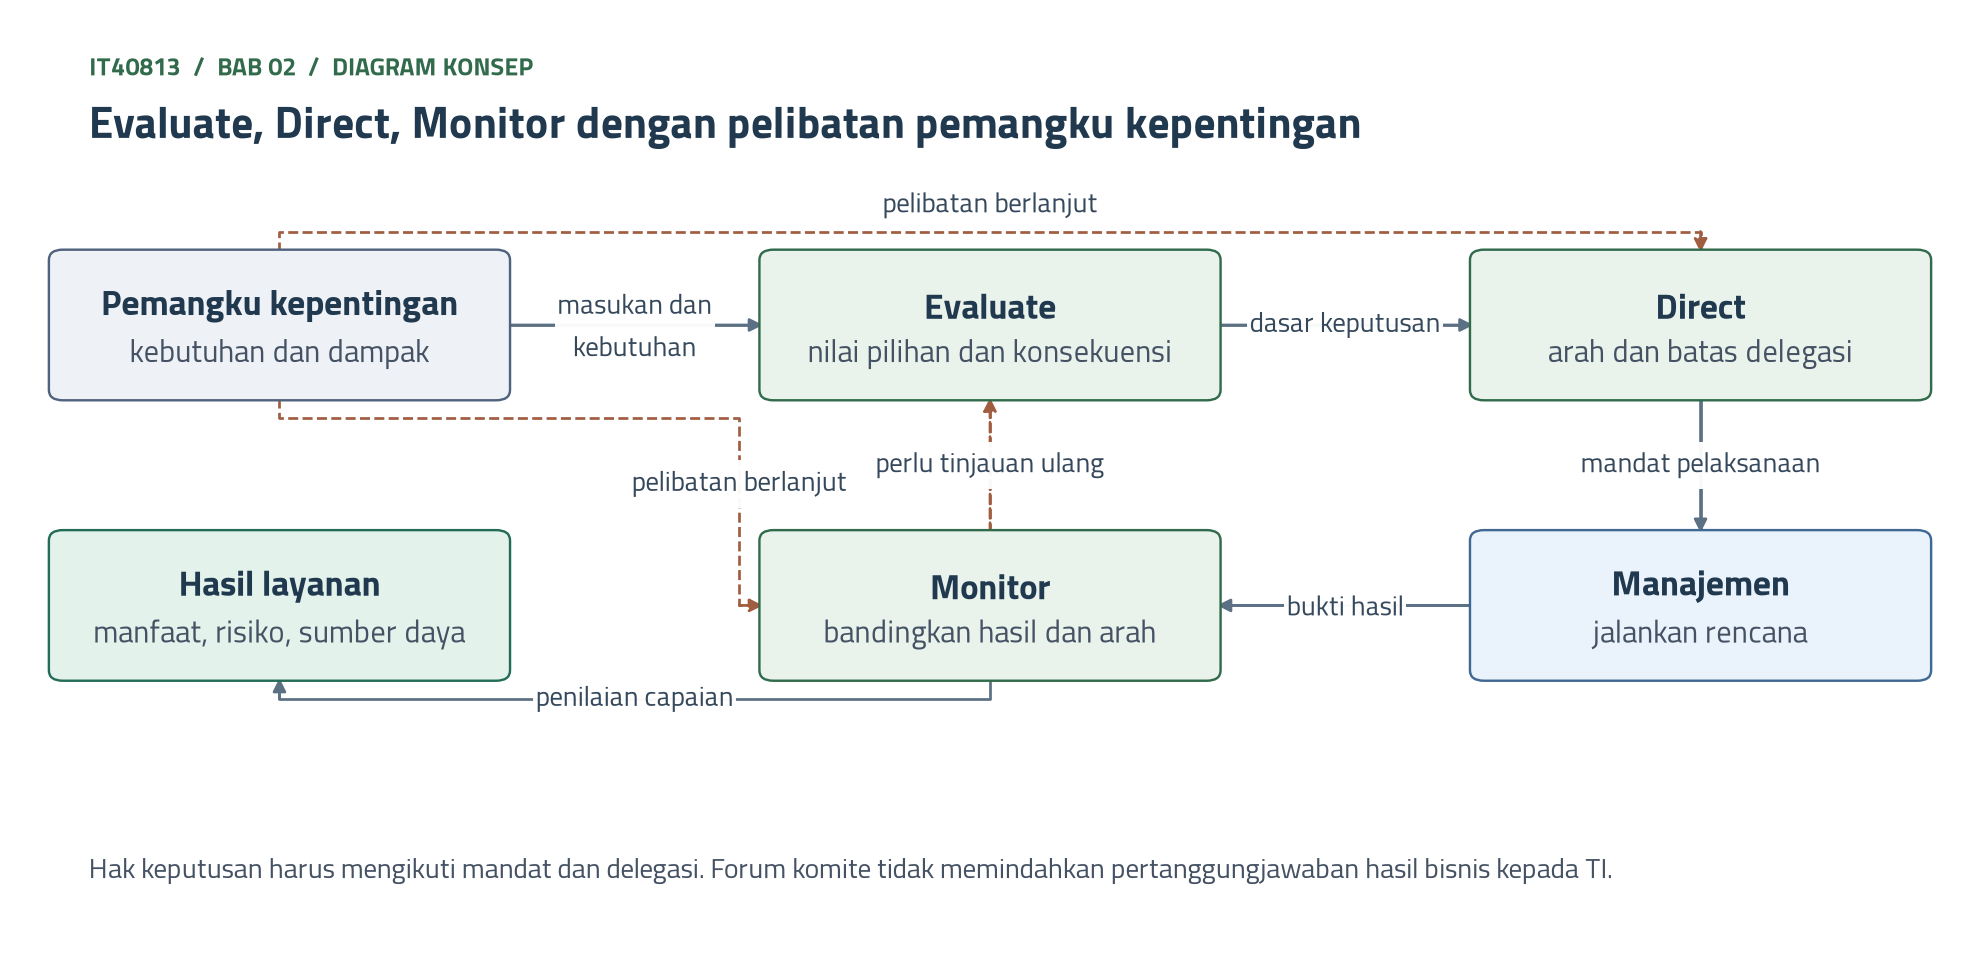
\includegraphics[width=0.96\textwidth,height=0.77\textheight,keepaspectratio]{../../figures/ch02-diagram-konsep.png}
  \label{fig:session02-ilustrasi-bab}
\end{frame}

\section{Tata Kelola Korporat}

\begin{frame}{\hfill}
  \centering
  \Huge{\textbf{Tata Kelola Korporat\\dan Posisi TI}}
\end{frame}

\begin{frame}{{\Large Dua Organ Perseroan}}
  \vspace{4pt}
  \small
  \begin{itemize}
    \item Direksi menjalankan pengurusan dalam batas undang-undang dan anggaran dasar (UU 40/2007
          Pasal 92).
    \item Dewan komisaris mengawasi dan memberi nasihat kepada direksi (Pasal 108).
    \item Anggaran dasar dapat mewajibkan persetujuan dewan komisaris untuk perbuatan hukum
          tertentu (Pasal 117).
    \item Komite adalah forum. Kewenangan hukum tetap mengikuti mandat.
    \item Pasal menjadi titik awal penelusuran, bukan alasan menyalin struktur perusahaan lain.
  \end{itemize}
\end{frame}

\begin{frame}{{\Large Organ, Forum, dan Pemilik Hasil}}
  \centering
  \resizebox{!}{0.74\textheight}{\begin{tikzpicture}[
  kotak/.style={draw, rounded corners, align=center, text width=2.85cm,
    minimum height=1.15cm, font=\scriptsize, fill=blue!8},
  panah/.style={-{Stealth[length=2mm]}, thick},
  keterangan/.style={font=\tiny, align=center, inner sep=1pt}
]
  \node[kotak, fill=praditagreen!15] (komisaris) at (0, 4.5)
    {\textbf{Dewan Komisaris}\\{\tiny\mdseries mengawasi dan\\memberi nasihat}};
  \node[kotak, fill=praditagreen!15] (direksi) at (4.45, 4.5)
    {\textbf{Direksi}\\{\tiny\mdseries mengurus perseroan\\dan menetapkan delegasi}};
  \node[kotak, fill=orange!12] (komite) at (8.9, 4.5)
    {\textbf{Komite pengarah TI}\\{\tiny\mdseries forum bermandat,\\bukan organ perseroan}};
  \node[kotak] (pemilik) at (2.225, 2.25)
    {\textbf{Pemilik layanan}\\{\tiny\mdseries direktur pelayanan:\\manfaat dan risiko}};
  \node[kotak] (manajemen) at (6.675, 2.25)
    {\textbf{Manajemen TI}\\{\tiny\mdseries kepala TI:\\kesiapan dan operasi}};
  \node[kotak, fill=green!10] (hasil) at (2.225, 0)
    {\textbf{Hasil layanan}\\{\tiny\mdseries waktu tunggu,\\mutu, dan biaya}};
  \node[kotak] (vendor) at (6.675, 0)
    {\textbf{Vendor}\\{\tiny\mdseries menjalankan pekerjaan\\sesuai kontrak}};
  \draw[panah] ([yshift=2mm]komisaris.east) -- node[keterangan, above]
    {pengawasan\\nasihat} ([yshift=2mm]direksi.west);
  \draw[panah] ([yshift=-2mm]direksi.west) -- node[keterangan, below]
    {laporan} ([yshift=-2mm]komisaris.east);
  \draw[panah] ([yshift=2mm]direksi.east) -- node[keterangan, above]
    {mandat} ([yshift=2mm]komite.west);
  \draw[panah] ([yshift=-2mm]komite.west) -- node[keterangan, below]
    {rekomendasi} ([yshift=-2mm]direksi.east);
  \draw[panah] (direksi.south) -- node[keterangan, fill=white] {delegasi}
    (pemilik.north);
  \draw[panah] (direksi.south) -- node[keterangan, fill=white] {delegasi}
    (manajemen.north);
  \draw[{Stealth[length=2mm]}-{Stealth[length=2mm]}, thick] (pemilik) --
    node[keterangan, above] {kebutuhan\\kesiapan} (manajemen);
  \draw[panah] (pemilik) -- node[keterangan, right] {memiliki\\manfaat} (hasil);
  \draw[panah] (manajemen) -- node[keterangan, right] {mengelola\\kontrak} (vendor);
  \draw[panah] (vendor) -- node[keterangan, above] {pekerjaan} (hasil);
\end{tikzpicture}
}
\end{frame}

\begin{frame}{{\Large Analogi dan Dua Contoh}}
  \vspace{4pt}
  \small
  \begin{itemize}
    \item Analogi: penasihat membantu menilai mutu bangunan, tetapi tanda tangan kontrak tetap
          mengikuti kewenangan pengelola rumah sakit.
    \item Misalkan pengadaan di atas Rp5 miliar perlu persetujuan dewan komisaris. Rp8 miliar
          melewati batas itu.
    \item Dewan komisaris menerima laporan risiko setiap triwulan, atau 4 kali setahun.
    \item Misalkan direktur pelayanan memiliki manfaat. Waktu tunggu dipengaruhi jadwal sekitar
          640 dokter.
    \item Kepala TI memimpin 52 staf TI, tetapi tidak berwenang mengubah jadwal dokter.
  \end{itemize}
\end{frame}

\begin{frame}{{\Large Pemetaan Kerja pada Dua Organ}}
  \vspace{4pt}
  \footnotesize
  \begin{tabularx}{\textwidth}{|>{\raggedright\arraybackslash}p{0.17\textwidth}|>{\raggedright\arraybackslash}X|>{\raggedright\arraybackslash}X|}
    \hline
    \textbf{Tugas} & \textbf{Direksi} & \textbf{Dewan komisaris} \\ \hline
    \textit{Evaluate} & Menilai opsi investasi dan dampaknya & Memberi nasihat; menyetujui bila
    anggaran dasar menetapkan \\ \hline
    \textit{Direct} & Menetapkan arah, pemilik manfaat, dan batas delegasi & Tidak memberi perintah
    operasional \\ \hline
    \textit{Monitor} & Memantau hasil dan memerintahkan koreksi & Mengawasi kebijakan dan jalannya
    pengurusan \\ \hline
    Pelibatan & Mengatur saluran masukan pasien, klinisi, dan unit lokal & Menanyakan apakah pihak
    terdampak sudah didengar \\ \hline
  \end{tabularx}

  \vspace{6pt}
  \small Pemetaan ini penafsiran bab, bukan isi standar. Cocokkan dengan anggaran dasar.
\end{frame}

\begin{frame}{{\Large Akuntabilitas Tidak Ikut Berpindah}}
  \vspace{4pt}
  \small
  \begin{itemize}
    \item Direksi bertanggung jawab atas pengurusan, dewan komisaris atas pengawasan (Pasal 97 dan
          Pasal 114).
    \item IIA: alih daya tidak mengubah akuntabilitas \textit{board} atas kegiatan asurans dan
          nasihat. Bab ini memakai logika serupa untuk vendor.
    \item Konsekuensi pertama: notulen berisi opsi, alasan, dan deklarasi kepentingan membantu
          menunjukkan kehati-hatian.
    \item Konsekuensi kedua: kontrak menetapkan tugas vendor, tetapi organisasi tetap menentukan
          siapa memantau hasil.
    \item Data latihan Bab 1: kontrak selesai, akun tetap aktif, 1.240 rekam kunjungan terbaca.
  \end{itemize}
\end{frame}

\section{ISO/IEC 38500 dan EDM}

\begin{frame}{\hfill}
  \centering
  \Huge{\textbf{ISO/IEC 38500:2024\\dan Model\\Evaluate, Direct, Monitor}}
\end{frame}

\begin{frame}{{\Large Perbedaan Edisi 2015 dan Edisi 2024}}
  \vspace{4pt}
  \footnotesize
  \begin{tabularx}{\textwidth}{|>{\raggedright\arraybackslash}p{0.17\textwidth}|>{\raggedright\arraybackslash}X|>{\raggedright\arraybackslash}X|}
    \hline
    \textbf{Aspek} & \textbf{Edisi 2015} & \textbf{Edisi 2024} \\ \hline
    Prinsip & Enam: tanggung jawab, strategi, akuisisi, kinerja, kesesuaian, perilaku manusia &
    Sebelas, mengikuti prinsip ISO 37000 \\ \hline
    Model & \textit{Evaluate}, \textit{Direct}, dan \textit{Monitor} oleh badan pengarah & Ditambah
    pelibatan pemangku kepentingan, di atas manajemen TI \\ \hline
    Letak tata kelola & Terutama pada badan pengarah & Di seluruh organisasi, dalam kerangka dari
    badan pengarah \\ \hline
    Kerangka & Konsepnya pertama muncul pada ISO/IEC 38502 & Enam unsur: arah, kapabilitas, kebijakan,
    delegasi, kinerja, akuntabilitas \\ \hline
  \end{tabularx}
\end{frame}

\begin{frame}{{\Large Sebelas Prinsip Edisi 2024}}
  \vspace{4pt}
  \small
  \begin{itemize}
    \item \textbf{Utama:} tujuan.
    \item \textbf{Dasar:} pembentukan nilai, strategi, pengawasan, dan akuntabilitas.
    \item \textbf{Pemungkin:} pelibatan pemangku kepentingan, kepemimpinan, data dan keputusan, tata
          kelola risiko, tanggung jawab sosial, serta kelangsungan dan kinerja dari waktu ke waktu.
    \item Daftar enam prinsip edisi 2015 tidak boleh diberi label edisi 2024.
    \item Rincian mengikuti \textit{white paper} di situs komite, bukan teks standar yang berbayar.
  \end{itemize}
\end{frame}

\begin{frame}{{\Large Tiga Tugas dan Satu Pelibatan}}
  \vspace{4pt}
  \small
  \begin{itemize}
    \item \textit{Evaluate}: memerlukan alternatif nyata, termasuk menunda atau menghentikan.
    \item \textit{Direct}: batas biaya, pemilik manfaat, risiko yang diterima, dan kondisi
          penghentian.
    \item \textit{Monitor}: membandingkan hasil dengan arahan dan dapat memicu evaluasi ulang.
    \item Pelibatan: pihak yang memakai layanan dan menanggung akibat memiliki saluran masukan.
    \item Analogi: panitia renovasi sekolah membandingkan pilihan, menetapkan batas, lalu memeriksa
          penggunaan ruangan.
  \end{itemize}
\end{frame}

\begin{frame}{{\Large Siklus EDM pada Keputusan Medikara+}}
  \centering
  \vspace{6pt}
  \resizebox{0.96\textwidth}{!}{\begin{tikzpicture}[
  kotak/.style={draw, rounded corners, align=center, text width=2.85cm,
    minimum height=1.25cm, font=\scriptsize, fill=blue!8},
  panah/.style={-{Stealth[length=2mm]}, thick},
  keterangan/.style={font=\tiny, align=center, inner sep=1pt}
]
  \node[kotak, fill=praditagreen!15] (pemangku) at (0, 2.6)
    {\textbf{Pemangku}\\\textbf{kepentingan}\\{\tiny\mdseries kebutuhan dan
    dampak:\\pasien, klinisi, unit lokal}};
  \node[kotak] (evaluate) at (4.4, 2.6)
    {\textbf{\textit{Evaluate}}\\{\tiny\mdseries nilai pilihan dan konsekuensi:\\Rp8
    miliar atau Rp6 miliar}};
  \node[kotak] (direct) at (8.8, 2.6)
    {\textbf{\textit{Direct}}\\{\tiny\mdseries arah dan batas delegasi:\\batas Rp8,8
    miliar,\\target 25 menit}};
  \node[kotak] (manajemen) at (8.8, 0)
    {\textbf{Manajemen}\\{\tiny\mdseries jalankan rencana:\\pemasangan di 5 rumah
    sakit}};
  \node[kotak, fill=orange!12] (monitor) at (4.4, 0)
    {\textbf{\textit{Monitor}}\\{\tiny\mdseries bandingkan hasil dan arah:\\38 menit,
    target 25 menit}};
  \node[kotak, fill=green!10] (hasil) at (0, 0)
    {\textbf{Hasil layanan}\\{\tiny\mdseries manfaat, risiko, sumber daya:\\baru 13,3
    persen target}};
  \draw[panah] (pemangku) -- node[keterangan, above]
    {masukan\\dan\\kebutuhan} (evaluate);
  \draw[panah] (evaluate) -- node[keterangan, above]
    {dasar\\keputusan} (direct);
  \draw[panah] (direct) -- node[keterangan, right]
    {mandat\\pelaksanaan} (manajemen);
  \draw[panah] (manajemen) -- node[keterangan, above]
    {bukti\\hasil} (monitor);
  \draw[panah] (monitor) -- node[keterangan, above]
    {penilaian\\capaian} (hasil);
  \draw[panah, dashed] (monitor) -- node[keterangan, right]
    {perlu\\tinjauan\\ulang} (evaluate);
  \draw[panah, densely dotted] (pemangku.south east) -- (monitor.north west);
  \draw[panah, densely dotted] (pemangku.north) -- ++(0, 0.42) -|
    node[keterangan, above, pos=0.25] {pelibatan berlanjut pada ketiga tugas}
    (direct.north);
\end{tikzpicture}
}
\end{frame}

\begin{frame}{{\Large Dua Contoh Berangka}}
  \vspace{4pt}
  \small
  \begin{itemize}
    \item Misalkan opsi Rp8 miliar dan Rp6 miliar dengan masa pakai 5 tahun: Rp1,6 miliar dan Rp1,2
          miliar per tahun.
    \item Dengan 336.000 janji temu per tahun: sekitar Rp4.760 dan Rp3.570 per janji temu.
    \item Target turun 15 menit dan 10 menit: sekitar Rp19.000 dan Rp21.400 per jam yang dihemat.
    \item Misalkan batas biaya Rp8,8 miliar (toleransi 10 persen). Hasil 38 menit berarti baru 13,3
          persen target.
    \item Kenaikan 27 persen, rata-rata pada Bab 1, berarti Rp10,16 miliar. Keputusan kembali ke
          direksi.
  \end{itemize}
\end{frame}

\begin{frame}{{\Large Dua Pemantauan yang Sering Tertukar}}
  \vspace{4pt}
  \small
  \begin{itemize}
    \item Manajemen memantau jalannya pekerjaan agar rencana terlaksana.
    \item Badan pengarah memantau apakah arah masih benar dan hasilnya sesuai.
    \item Misalkan 5 rumah sakit mengirim laporan pekanan: 260 laporan setahun untuk manajemen.
    \item Direksi menerima 4 laporan triwulan: hasil, risiko, dan keputusan yang diperlukan.
    \item COBIT juga memisahkan keduanya. Bab 4 membahas rinciannya.
  \end{itemize}
\end{frame}

\section{Hak Keputusan TI}

\begin{frame}{\hfill}
  \centering
  \Huge{\textbf{Hak Keputusan TI}}
\end{frame}

\begin{frame}{{\Large Lima Keputusan, Enam Arketipe}}
  \vspace{4pt}
  \small
  \begin{itemize}
    \item Hak keputusan: siapa memberi masukan dan siapa menetapkan keputusan akhir.
    \item Weill: lebih dari 250 perusahaan di 23 negara.
    \item Lima keputusan: prinsip TI, arsitektur, infrastruktur, kebutuhan aplikasi bisnis, serta
          investasi dan prioritas.
    \item Perusahaan unggul pada pertumbuhan lebih terdesentralisasi; unggul pada laba lebih terpusat.
    \item Tidak ada satu susunan terbaik. Letak keputusan mengikuti tujuan kinerja.
  \end{itemize}
\end{frame}

\begin{frame}{{\Large Enam Arketipe pada Medikara}}
  \vspace{2pt}
  \scriptsize
  \begin{tabularx}{\textwidth}{|>{\raggedright\arraybackslash}p{0.14\textwidth}|>{\raggedright\arraybackslash}p{0.2\textwidth}|>{\raggedright\arraybackslash}X|>{\raggedright\arraybackslash}X|}
    \hline
    \textbf{Arketipe} & \textbf{Letak keputusan} & \textbf{Misalkan di Medikara} & \textbf{Akibat} \\ \hline
    Monarki bisnis & Pimpinan bisnis senior & Direksi memutuskan prinsip identitas pasien & Arah kuat;
    perlu masukan kelayakan \\ \hline
    Monarki TI & Pimpinan TI & Kepala TI memutuskan standar integrasi & Standar konsisten; manfaat
    layanan kurang terwakili \\ \hline
    Feodal & Tiap unit bisnis & Tiap rumah sakit memilih sistem sendiri & Cepat di tingkat lokal; 5
    versi SIMRS sulit disatukan \\ \hline
    Federal & Pusat bersama unit & Direktur pelayanan bersama 5 direktur rumah sakit & Pusat dan unit
    terwakili; kesepakatan lebih lama \\ \hline
    Duopoli TI & TI bersama satu kelompok bisnis & Kepala TI bersama direktur pelayanan & Nilai dan
    kelayakan dinilai bersama; perlu aturan bila tidak sepakat \\ \hline
    Anarki & Individu atau kelompok kecil & Unit menyusun laporan dengan \textit{spreadsheet} sendiri &
    Murah di awal; data tersebar \\ \hline
  \end{tabularx}
\end{frame}

\begin{frame}{{\Large Matriks Hak Keputusan Medikara}}
  \centering
  \resizebox{!}{0.7\textheight}{\begin{tikzpicture}[
  kolom/.style={font=\scriptsize\bfseries, align=center, text width=1.28cm},
  baris/.style={font=\scriptsize, align=left, text width=3.1cm, anchor=west},
  pemutus/.style={circle, fill=praditagreen, draw=black, minimum size=3mm,
    inner sep=0pt},
  masukan/.style={circle, fill=white, draw=black, thick, minimum size=3mm,
    inner sep=0pt},
  kini/.style={rectangle, fill=red!22, draw=black, minimum size=2.8mm,
    inner sep=0pt}
]
  % Kisi 6 kolom arketipe dan 5 baris keputusan; lebar total 11,7 cm.
  \fill[praditagreen!15] (0, 0) rectangle (11.7, 0.85);
  \draw[gray] (0, -3.5) grid[xstep=11.7, ystep=0.7] (11.7, 0);
  \foreach \posisi in {3.3, 4.7, 6.1, 7.5, 8.9, 10.3, 11.7} {
    \draw[gray] (\posisi, -3.5) -- (\posisi, 0.85);
  }
  \draw[gray] (0, -3.5) rectangle (11.7, 0.85);
  \node[baris, font=\scriptsize\bfseries] at (0, 0.425) {Keputusan};
  \node[kolom] at (4.0, 0.425) {Monarki bisnis};
  \node[kolom] at (5.4, 0.425) {Monarki TI};
  \node[kolom] at (6.8, 0.425) {Feodal};
  \node[kolom] at (8.2, 0.425) {Federal};
  \node[kolom] at (9.6, 0.425) {Duopoli TI};
  \node[kolom] at (11.0, 0.425) {Anarki};
  \node[baris] at (0, -0.35) {Prinsip TI};
  \node[baris] at (0, -1.05) {Arsitektur TI};
  \node[baris] at (0, -1.75) {Infrastruktur TI};
  \node[baris] at (0, -2.45) {Kebutuhan aplikasi bisnis};
  \node[baris] at (0, -3.15) {Investasi dan prioritas TI};
  % Prinsip TI
  \node[pemutus] at (4.0, -0.35) {};
  \node[masukan] at (8.2, -0.35) {};
  \node[kini] at (5.4, -0.35) {};
  % Arsitektur TI
  \node[pemutus] at (5.4, -1.05) {};
  \node[masukan] at (8.2, -1.05) {};
  \node[kini] at (6.8, -1.05) {};
  % Infrastruktur TI
  \node[pemutus] at (5.4, -1.75) {};
  \node[masukan] at (9.6, -1.75) {};
  \node[kini] at (6.8, -1.75) {};
  % Kebutuhan aplikasi bisnis
  \node[pemutus] at (8.2, -2.45) {};
  \node[masukan] at (6.55, -2.45) {};
  \node[kini] at (7.05, -2.45) {};
  % Investasi dan prioritas TI
  \node[pemutus] at (4.0, -3.15) {};
  \node[masukan] at (9.6, -3.15) {};
  \node[kini] at (5.4, -3.15) {};
  % Keterangan penanda
  \node[pemutus] at (0.2, -3.95) {};
  \node[font=\scriptsize, anchor=west] at (0.4, -3.95) {pemutus usulan};
  \node[masukan] at (3.6, -3.95) {};
  \node[font=\scriptsize, anchor=west] at (3.8, -3.95) {pemberi masukan usulan};
  \node[kini] at (7.9, -3.95) {};
  \node[font=\scriptsize, anchor=west] at (8.1, -3.95) {pemutus saat ini};
\end{tikzpicture}
}
\end{frame}

\begin{frame}{{\Large Masukan, Veto, dan Keputusan Akhir}}
  \vspace{4pt}
  \small
  \begin{itemize}
    \item Masukan wajib didengar, tetapi boleh tidak diikuti dengan alasan tertulis.
    \item Veto menghentikan keputusan, sehingga harus eksplisit dan dibatasi.
    \item Misalkan 4 pihak memegang veto dan tiap pihak menyetujui 90 persen usulan: hanya 65,6 persen
          usulan lolos.
    \item Analogi: banyak peserta menyampaikan alergi, tetapi satu koordinator mengonfirmasi pesanan.
    \item Misalkan 5 rumah sakit membeli identitas sendiri: Rp3,5 miliar, melawan platform bersama Rp2
          miliar.
  \end{itemize}
\end{frame}

\begin{frame}{{\Large Contoh Batas Delegasi}}
  \vspace{4pt}
  \footnotesize
  \begin{tabularx}{\textwidth}{|>{\raggedright\arraybackslash}p{0.3\textwidth}|>{\raggedright\arraybackslash}X|>{\raggedright\arraybackslash}p{0.27\textwidth}|}
    \hline
    \textbf{Nilai keputusan} & \textbf{Pemutus akhir} & \textbf{Laporan} \\ \hline
    Sampai Rp100 juta & Kepala TI, dengan masukan pemilik layanan & Ringkasan triwulan ke komite \\ \hline
    Di atas Rp100 juta sampai Rp400 juta & Komite pengarah TI, sesuai mandat direksi & Notulen ke direksi
    \\ \hline
    Di atas Rp400 juta sampai Rp5 miliar & Direksi & Laporan triwulan ke dewan komisaris \\ \hline
    Di atas Rp5 miliar & Direksi dengan persetujuan dewan komisaris, bila anggaran dasar menetapkan &
    Laporan triwulan ke dewan komisaris \\ \hline
    Kenaikan di atas 10 persen & Kembali ke pemutus awal & Alasan dan pilihan koreksi \\ \hline
  \end{tabularx}

  \vspace{4pt}
  \small Semua angka pengandaian, bukan batas hukum.
\end{frame}

\begin{frame}{{\Large Kasus Medikara: Siapa Mencabut Akun Vendor?}}
  \vspace{4pt}
  \small
  \begin{itemize}
    \item R-01: audit memeriksa 30 dari 120 akun vendor, 6 akun aktif setelah penugasan berakhir.
    \item Bulan berikutnya 24 akun dicabut. Siapa yang berwenang?
    \item Misalkan pemilik Medikara+ memutuskan akses, dengan masukan kepala TI. Bila kepala TI
          keberatan, naik ke direktur pelayanan.
    \item Staf TI mencabut akun paling lambat 1 hari kerja setelah penugasan berakhir.
    \item Direksi menerima risiko sisa R-01. Audit internal memeriksa kontrol AC-01.
  \end{itemize}
\end{frame}

\section{Struktur dan Komite}

\begin{frame}{\hfill}
  \centering
  \Huge{\textbf{Struktur, Proses,\\dan Mekanisme Relasional}}
\end{frame}

\begin{frame}{{\Large Tiga Mekanisme Tata Kelola}}
  \centering
  \resizebox{!}{0.7\textheight}{\begin{tikzpicture}[
  kotak/.style={draw, rounded corners, align=center, text width=3.3cm,
    minimum height=1.3cm, font=\scriptsize, fill=blue!8},
  masalah/.style={draw, rounded corners, align=center, text width=3.3cm,
    minimum height=0.75cm, font=\scriptsize, fill=red!22},
  panah/.style={-{Stealth[length=2mm]}, thick},
  keterangan/.style={font=\tiny, align=center, inner sep=1pt}
]
  \node[masalah] (masalah1) at (0, 4.0) {Bila hilang:\\keputusan tanpa pemutus};
  \node[masalah] (masalah2) at (4.0, 4.0) {Bila hilang:\\keputusan tidak ditinjau};
  \node[masalah] (masalah3) at (8.0, 4.0) {Bila hilang:\\piagam hanya tersimpan};
  \node[kotak] (struktur) at (0, 2.1)
    {\textbf{Struktur}\\{\tiny\mdseries forum, peran, mandat,\\dan batas delegasi}};
  \node[kotak] (proses) at (4.0, 2.1)
    {\textbf{Proses}\\{\tiny\mdseries agenda EDM, catatan keputusan,\\dan peninjauan
    manfaat}};
  \node[kotak] (relasional) at (8.0, 2.1)
    {\textbf{Mekanisme relasional}\\{\tiny\mdseries dialog lintas fungsi, bahasa
    bersama,\\dan belajar dari insiden}};
  \node[draw, rounded corners, align=center, fill=green!10, font=\scriptsize,
    text width=11.1cm, minimum height=0.9cm] (hasil) at (4.0, 0)
    {\textbf{Keputusan yang dijalankan dan dapat diperiksa}\\{\tiny\mdseries satu
    pemutus, alasan tercatat, tindak lanjut selesai, dan hasil layanan ditinjau}};
  \draw[panah, dashed] (struktur) -- (masalah1);
  \draw[panah, dashed] (proses) -- (masalah2);
  \draw[panah, dashed] (relasional) -- (masalah3);
  \draw[panah] (struktur) -- (struktur |- hasil.north);
  \draw[panah] (proses) -- (proses |- hasil.north);
  \draw[panah] (relasional) -- (relasional |- hasil.north);
\end{tikzpicture}
}
\end{frame}

\begin{frame}{{\Large Dua Contoh Mekanisme}}
  \vspace{4pt}
  \small
  \begin{itemize}
    \item Misalkan komite bertemu sebulan sekali dengan 96 item agenda setahun.
    \item Sebanyak 72 item (75 persen) berupa laporan, hanya 24 item (25 persen) meminta keputusan.
    \item Misalkan ada 60 permintaan perubahan per bulan, 48 di antaranya berisiko rendah.
    \item Menunggu rapat bulanan: rata-rata sekitar 15 hari. Dengan delegasi 2 hari: rata-rata 4,6 hari.
    \item Analogi: bagan piket tidak cukup bila petugas tidak mau melaporkan masalah.
  \end{itemize}
\end{frame}

\begin{frame}{{\Large Piagam Komite Pengarah TI}}
  \vspace{2pt}
  \footnotesize
  \renewcommand{\arraystretch}{1.15}
  \begin{tabularx}{\textwidth}{|>{\raggedright\arraybackslash}p{0.2\textwidth}|>{\raggedright\arraybackslash}X|}
    \hline
    \textbf{Unsur} & \textbf{Misalkan di Medikara} \\ \hline
    Anggota & 9 orang: direktur utama sebagai ketua, direktur pelayanan, direktur keuangan, kepala TI, 2
    direktur rumah sakit bergilir, kepala rekam medis, kepala risiko, dan hukum \\ \hline
    Mandat & Memutuskan sampai Rp400 juta; merekomendasikan di atasnya kepada direksi \\ \hline
    Kuorum & 6 dari 9 anggota, dan pemilik risiko yang dibahas wajib hadir \\ \hline
    Rapat & Bulanan selama 2 jam, serta rapat insiden sesuai jalur eskalasi \\ \hline
    Konflik kepentingan & Anggota menyatakan hubungan dengan vendor; vendor tanpa hak memutus \\ \hline
    Eskalasi & Keputusan di luar mandat naik ke direksi; keputusan darurat dicatat dan ditinjau \\ \hline
    Laporan & Notulen keputusan ke direksi dan ringkasan triwulan untuk pengawasan \\ \hline
  \end{tabularx}
\end{frame}

\begin{frame}{{\Large Struktur Mengikuti Ukuran dan Konteks}}
  \vspace{4pt}
  \footnotesize
  \begin{tabularx}{\textwidth}{|>{\raggedright\arraybackslash}p{0.3\textwidth}|>{\raggedright\arraybackslash}X|>{\raggedright\arraybackslash}X|}
    \hline
    \textbf{Organisasi} & \textbf{Forum yang masuk akal} & \textbf{Risiko yang perlu dijaga} \\ \hline
    Klinik mitra: 60 karyawan, 2 staf TI & Agenda TI triwulan pada rapat pimpinan yang sudah ada & Satu
    orang memegang semua keputusan \\ \hline
    Jaringan menengah: 800 karyawan, 15 staf TI & Komite kecil dua bulanan dengan mandat tertulis & Forum
    berubah menjadi laporan kemajuan \\ \hline
    Medikara: sekitar 4.800 karyawan, 52 staf TI & Komite bulanan dan forum arsitektur berdelegasi &
    Antrean keputusan dan jarak dengan unit lokal \\ \hline
  \end{tabularx}

  \vspace{6pt}
  \small Medikara: 216 jam orang per tahun, 0,045 jam per karyawan. Klinik mitra: 120 jam orang, 2 jam
  per karyawan.
\end{frame}

\begin{frame}{{\Large Kasus Medikara: Komite yang Berani Meninjau}}
  \vspace{4pt}
  \small
  \begin{itemize}
    \item Laporan: 90 persen pekerjaan, tanpa ukuran waktu tunggu. Komite meminta opsi koreksi.
    \item Pilihan pertama: lanjut tanpa perubahan, waktu tunggu tetap sekitar 38 menit.
    \item Pilihan kedua: ubah alur dan jadwal petugas, tambah Rp400 juta, total Rp8,4 miliar.
    \item Pilihan ketiga: tunda pemasangan pada 18 klinik.
    \item Keputusan: pilihan kedua. Bila belum di bawah 30 menit dalam 90 hari, direksi mengevaluasi
          ulang.
  \end{itemize}
\end{frame}

\section{Keselarasan dan Nilai}

\begin{frame}{\hfill}
  \centering
  \Huge{\textbf{Keselarasan Bisnis dan TI\\serta Penciptaan Nilai}}
\end{frame}

\begin{frame}{{\Large Keselarasan dan Hitungan Manfaat}}
  \vspace{2pt}
  \footnotesize
  \begin{itemize}
    \item Keselarasan: prioritas TI dan prioritas bisnis saling mendukung serta terus disesuaikan.
    \item Analogi: kendaraan baru tidak menolong bila alamat pengantaran tetap salah.
  \end{itemize}
  \vspace{2pt}
  \begin{tabularx}{\textwidth}{|>{\raggedright\arraybackslash}X|>{\raggedright\arraybackslash}p{0.25\textwidth}|>{\raggedright\arraybackslash}p{0.25\textwidth}|}
    \hline
    \textbf{Ukuran} & \textbf{Target} & \textbf{Hasil tiga bulan} \\ \hline
    Waktu tunggu & 25 menit & 38 menit \\ \hline
    Capaian terhadap target & 100 persen & 13,3 persen \\ \hline
    Jam tunggu yang dihemat per tahun & 84.000 jam & 11.200 jam \\ \hline
    Biaya per jam yang dihemat & sekitar Rp19.000 & sekitar Rp143.000 \\ \hline
  \end{tabularx}
\end{frame}

\begin{frame}{{\Large Rantai Tata Kelola, Keselarasan, dan Kinerja}}
  \centering
  \resizebox{!}{0.74\textheight}{\begin{tikzpicture}[
  kotak/.style={draw, rounded corners, align=center, text width=2.95cm,
    minimum height=1.15cm, font=\scriptsize, fill=blue!8},
  panah/.style={-{Stealth[length=2mm]}, thick},
  keterangan/.style={font=\tiny, align=center, inner sep=1pt}
]
  \node[kotak] (mekanisme) at (0, 2.4)
    {\textbf{Mekanisme tata kelola}\\{\tiny\mdseries struktur, proses, relasional}};
  \node[kotak, fill=orange!12] (keselarasan) at (4.2, 2.4)
    {\textbf{Keselarasan strategis}\\{\tiny\mdseries prioritas bisnis dan TI saling
    mendukung}};
  \node[kotak, fill=green!10] (kinerja) at (8.4, 2.4)
    {\textbf{Kinerja organisasi}\\{\tiny\mdseries hasil yang diukur}};
  \draw[panah] (mekanisme) -- (keselarasan);
  \draw[panah] (keselarasan) -- (kinerja);
  % Jalur langsung: letak perbedaan temuan antarpenelitian.
  \draw[panah, dashed] (mekanisme.north) -- ++(0, 0.62) -|
    node[keterangan, above, pos=0.25, text width=8.4cm]
    {Pengaruh langsung: Wu dkk. tidak menemukan sisa pengaruh (mediasi penuh);
    Turel dkk. masih menemukan sisa pada tingkat dewan (mediasi sebagian)}
    (kinerja.north);
  \node[draw, rounded corners, align=center, fill=red!22, font=\tiny,
    text width=2.95cm, minimum height=0.6cm] (gaya) at (8.4, 4.75)
    {Gaya tata kelola otoriter melemahkan pengaruh (Turel dkk.)};
  \draw[panah] (gaya.south) -- ++(0, -0.72);
  % Contoh pengandaian Medikara pada baris bawah.
  \node[kotak, fill=white] (mandat) at (0, 0)
    {\textbf{Medikara}\\{\tiny\mdseries mandat, komite, pemilik manfaat}};
  \node[kotak, fill=white] (target) at (4.2, 0)
    {\textbf{Target bersama}\\{\tiny\mdseries waktu tunggu 40 menjadi 25 menit}};
  \node[kotak, fill=white] (capaian) at (8.4, 0)
    {\textbf{Hasil tiga bulan}\\{\tiny\mdseries 38 menit, baru 13,3 persen target}};
  \draw[panah] (mandat) -- (target);
  \draw[panah] (target) -- (capaian);
  \draw[densely dotted, thick] (mekanisme) -- (mandat);
  \draw[densely dotted, thick] (keselarasan) -- (target);
  \draw[densely dotted, thick] (kinerja) -- (capaian);
\end{tikzpicture}
}
\end{frame}

\begin{frame}{{\Large Bukti Empiris dan Batasnya}}
  \vspace{2pt}
  \scriptsize
  \begin{tabularx}{\textwidth}{|>{\raggedright\arraybackslash}p{0.2\textwidth}|>{\raggedright\arraybackslash}p{0.21\textwidth}|>{\raggedright\arraybackslash}X|>{\raggedright\arraybackslash}p{0.21\textwidth}|}
    \hline
    \textbf{Sumber} & \textbf{Data} & \textbf{Temuan} & \textbf{Batas penerapan} \\ \hline
    Weill (2004) & Lebih dari 250 perusahaan, 23 negara & Letak hak keputusan mengikuti tujuan kinerja &
    Tidak khusus rumah sakit \\ \hline
    De Haes dan Van Grembergen (2009) & Beberapa strategi penelitian & Kematangan keselarasan lebih tinggi
    pada paduan praktik yang matang & Kajian eksploratif \\ \hline
    Huang dkk. (2010) & 3 organisasi kecil dan menengah & Komite dan komunikasi menjelaskan perbedaan hasil
    pemakaian TI & Berupa proposisi \\ \hline
    Gerow dkk. (2014) & Meta-analisis & Korelasi rata-rata keselarasan dengan kinerja positif & Korelasi,
    bukan sebab akibat \\ \hline
    Wu dkk. (2015) & 131 perusahaan Taiwan, 72 data arsip & Keselarasan memediasi penuh & Satu negara; survei
    \\ \hline
    Turel dkk. (2017) & Dua studi empiris & Keselarasan memediasi sebagian; gaya otoriter melemahkan & Tingkat
    dewan; perlu dipetakan ke dua organ \\ \hline
  \end{tabularx}
\end{frame}

\section{Aktivitas dan Latihan}

\begin{frame}{{\Large Aktivitas: Matriks Hak Keputusan dan Piagam}}
  \vspace{2pt}
  \small
  \begin{itemize}
    \item Daftar 8 sampai 10 keputusan TI, misalnya vendor SIMRS, anggaran keamanan, atau data ke mitra.
    \item Isi pemberi masukan, pemutus akhir, pengawas, batas delegasi, dan bukti.
    \item Bandingkan dengan arketipe, lalu tulis piagam komite pengarah TI.
    \item Uji piagam dengan satu keputusan investasi dan satu insiden mendesak.
    \item Luaran masuk C1. Berkas ada di \texttt{sources/chapter02/}.
  \end{itemize}
\end{frame}

\begin{frame}{{\Large Ringkasan}}
  \vspace{4pt}
  \small
  \begin{itemize}
    \item Tata kelola TI bagian dari tata kelola organisasi, mengikuti anggaran dasar dan delegasi.
    \item EDM menghubungkan pilihan, arahan, dan hasil. Edisi 2024 memakai sebelas prinsip dan menambah
          pelibatan pemangku kepentingan.
    \item Matriks memisahkan masukan dari keputusan akhir. Tidak ada satu susunan terbaik.
    \item Bentuk komite mengikuti ukuran dan konteks organisasi.
    \item Forum tata kelola bernilai ketika memperjelas keputusan dan menguji hasil layanan.
  \end{itemize}
\end{frame}

\begin{frame}{{\Large Latihan dan Bacaan}}
  \vspace{2pt}
  \footnotesize
  \begin{enumerate}
    \item Sebuah rumah sakit membentuk komite pengarah TI, tetapi rapatnya hanya membahas laporan
          kemajuan proyek. Bagian mana dari model \textit{Evaluate, Direct, Monitor} yang belum dijalankan?
          Jelaskan.
    \item Bandingkan dua arketipe hak keputusan untuk investasi aplikasi pasien Medikara+. Mana yang lebih
          tepat, dan apa \textit{trade-off}-nya?
    \item Ringkas temuan Wu, Straub, dan Liang (2015) tentang peran keselarasan strategis. Nilai apakah
          temuan itu berlaku untuk organisasi tempat bekerja.
  \end{enumerate}
  \vspace{4pt}
  \textbf{Bacaan:} \href{https://www.iso.org/standard/81684.html}{ISO/IEC 38500:2024};
  Weill dan Ross (2004); \href{https://aisel.aisnet.org/misq/vol39/iss2/12/}{Wu dkk. (2015)}.
\end{frame}

\end{document}
